\chapter{Introdução}
%---------------------
% Edite a partir daqui 
%---------------------
Para editar a introdução, edite o arquivo introdução.tex na pasta textuais. Para chamar uma entrada do \gls{gls} use \verb+\gls{rótulo}+, chamando a entrada apropriada no arquivo postextuais/glossarios.tex.

Atente que esse modelo pode ser aplicado tanto ao TCC 1 quanto ao TCC 2, entretanto eles tem conteúdo diferente: 

\begin{minipage}{0.5\textwidth}
Conteúdo exigido do TCC 1
\end{minipage}
\begin{minipage}{0.5\textwidth}
Conteúdo exigido do TCC 2
\end{minipage}
\begin{minipage}{0.5\textwidth}

	\vspace{-15mm}
	\begin{itemize}
		\item introdução
		\item Justificativa
		\item Problematização
		\item Hipótese
		\item Objetivos
		\item Revisão bibliográfica
		\item Metodologia 
		\item Cronograma
		\item Referências
		\item Apêndices (opcional)
		\item Anexos (opcional)				
	\end{itemize}
\end{minipage}
\begin{minipage}{0.5\textwidth}
	\vspace{1cm}
	\begin{itemize}
		\item introdução
		\item Justificativa
		\item Problematização
		\item Hipótese
		\item Objetivos
		\item Revisão bibliográfica
		\item Metodologia 
		\item Proposta de trabalho
		\item Resultados
		\item Discussão
		\item Conclusão
		\item Referências
		\item Apêndices (opcional)
		\item Anexos (opcional)
	\end{itemize}
\end{minipage}

Capa, contracapa, folha de aprovação, listas de figuras, tabelas e o sumário são todos automaticamente gerados pelo \LaTeX   com base no que for incluído nos arquivos. O título do capítulo sempre será o que estiver incluso no comando \verb|\chapter{}| no início de cada capitulo. 

Notas de rodapé são incluídas com o comando:\par
\verb|\footnote{Texto da nota de rodapé}|\footnote{O texto da nota de rodapé é automaticamente numerado}.

A estrutura de arquivos que podem ou não ser incluídos está na sessão textual do arquivo \verb|TCC.tex|. Para omitir algum arquivo coloque um \verb|%| no inicio da linha onde ele é referenciado. 

\begin{figure}[!htb]
	\centering 
	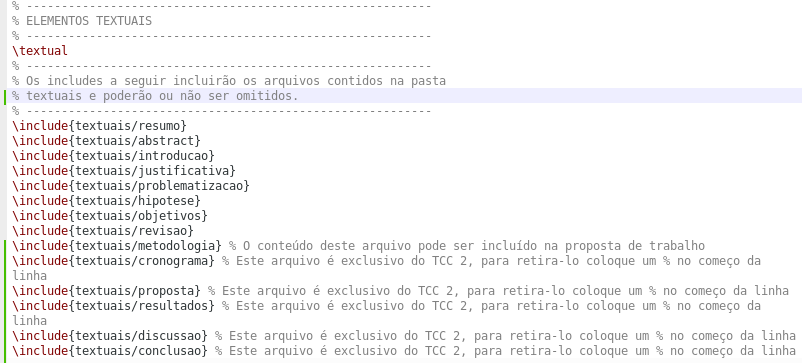
\includegraphics[width=0.8mm]{imagens/estrutura}
	\caption{Estrutura dos arquivos textuais}
	\label{fig:estrutura}
\end{figure}